\chapter{Introduction}\label{ch:introduction}

\vspace*{-50pt}

\begin{figure}[ht]
        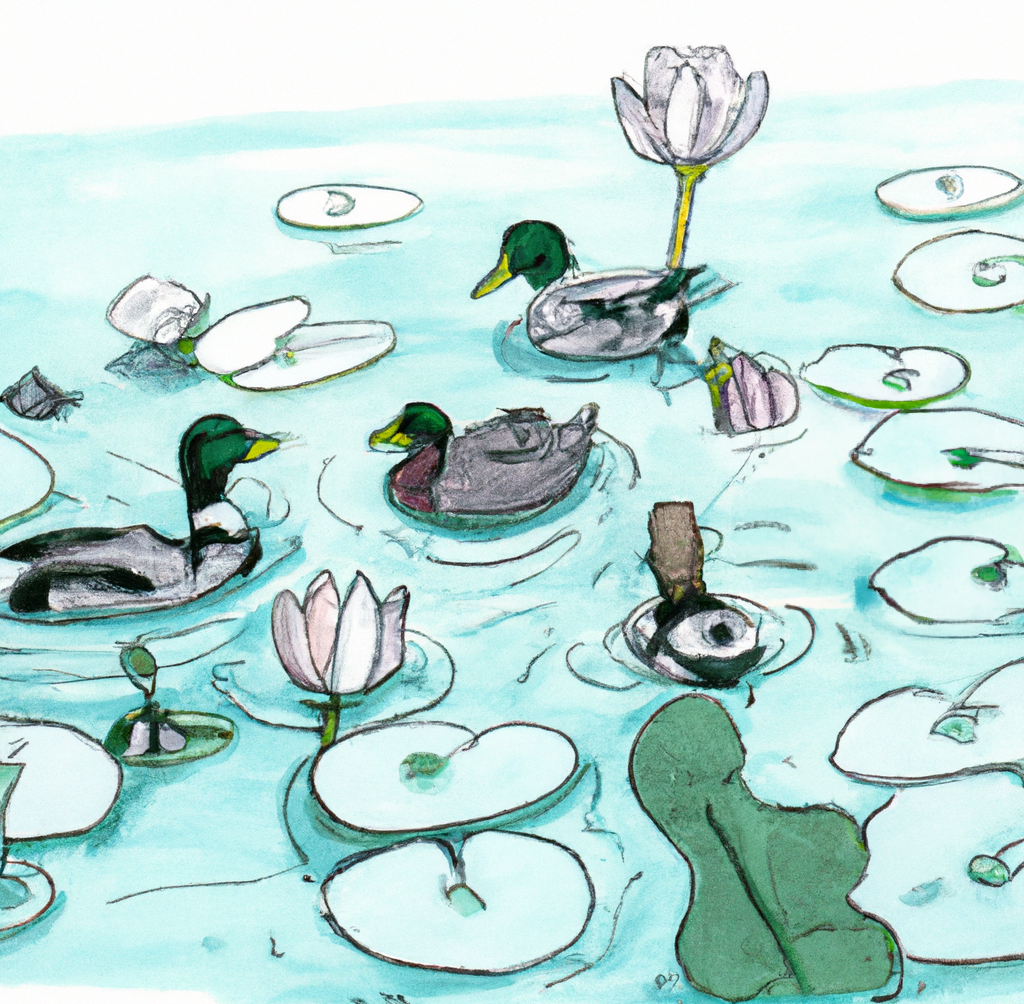
\includegraphics[width=0.35\textwidth, right]{img/dalle-ducks.png}
        \captionsetup{textformat=empty,labelformat=blank}
        \caption{Generated with Dall-E. \url{https://labs.openai.com/}. ``A duck dominating sitting on a sea rose''}
\end{figure}

\epigraph{\itshape We have seen [\ldots], which is to say, all meaning comes from analogies.}{Douglas Richard Hofstadter, \textit{I am A Strange Loop}}

Quack! Quack! They were careless for a second and immediately the dreaded \textit{geesiosi} clan has taken the opportunity and conquered your befriended ducks' \textit{Merganser Lake}!
Now they are sitting on all the beautiful water lilies refusing to give them back and the desperate ducks have asked for your assistance.
The ducks have given you a map of the lake (see the left side of \cref{fig:duck-lake}) where all the water lilies are marked in green.
You instantly assured them of your help and started to analyze the situation!

You quickly noticed that the \textit{geesiosi} members are very frightened of the ducks' quacking. 
One single duck can free up an entire water lily and even drive away all the geese on neighboring plants! After thinking about this for a few minutes you realized that this might indeed be the key observation to regaining the lake. 
After some more deep contemplating, you came up with a good assignment of ducks to water lilies, where only a minimal number of ducks is required to liberate the whole territory again.

Happy with your idea, you present it to the \textit{Supreme Duck Decision Board}, but unfortunately, you could not fully convince them and the \textit{Chief Strategy Duck} shared her worries with you: 
They know that they also have to hold the fort and protect the lake against another future rush of the \textit{geesiosi}.
This is going to be a very tedious task for the individuals because a duck has to sit alone on a water lily waiting all day. They would rather want to have at least someone around to quack with together!

%____
You suggest them to revise your solution making sure that there is always another friend sitting at most two water lilies away. After a short retreat, you came up with a new solution where only two warrior ducks (see the right side of \cref{fig:duck-lake}) are required and they only have one lily in between. 

Now the ducks were fully satisfied with the solution! But while the chosen two ducks were being sent out over the water's surface, you were still thinking about the problem.
It looked so easy at first, but in the end, you had to try all the possible configurations while playing around with the number of ducks used (of course you did not tell the ducks that it was that simple, because they now think you are a wizard!). 
You are wondering, whether there is a way to significantly reduce the number of configurations you have to try to find a solution.

\begin{figure}[t]
    \centering
    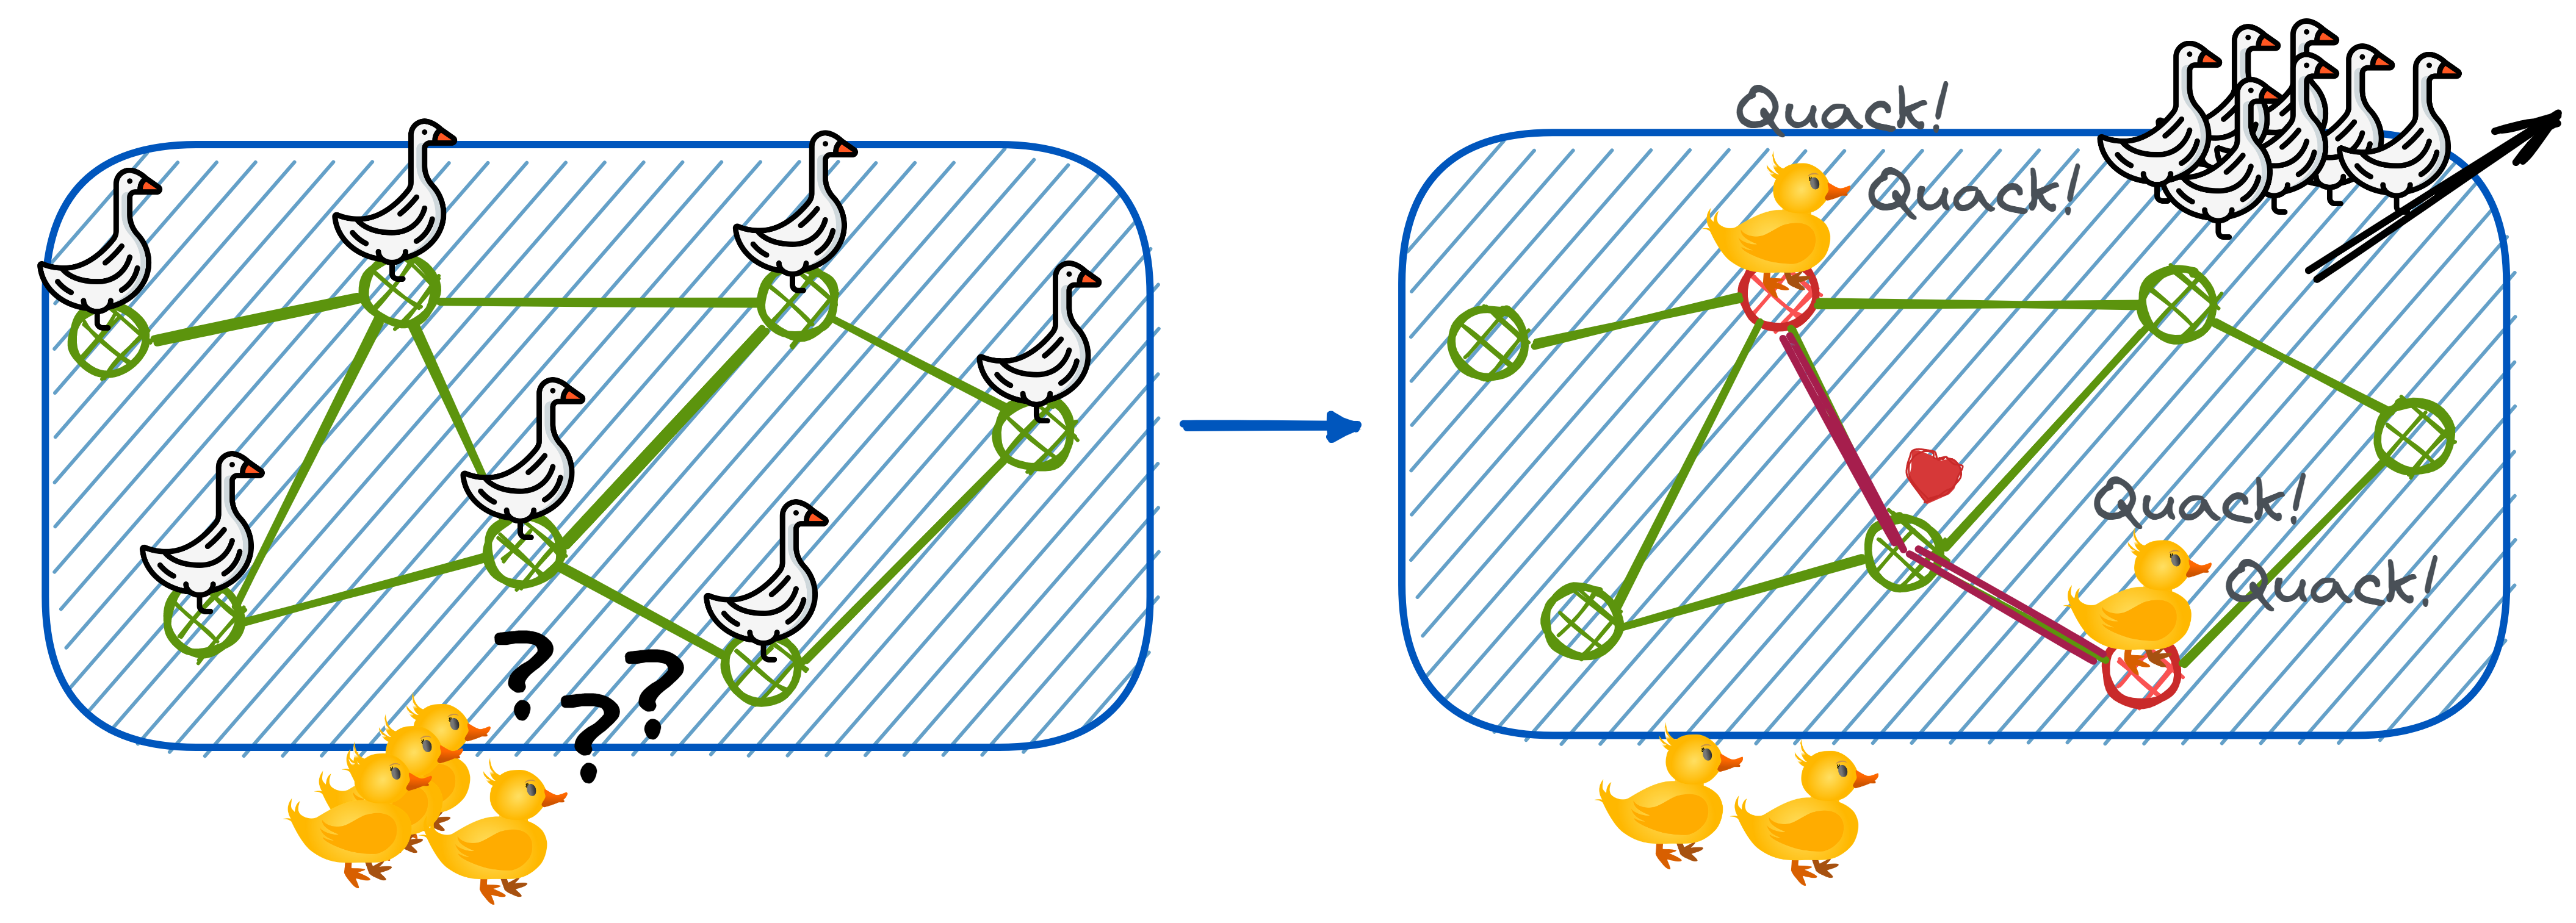
\includegraphics[width=0.9\columnwidth]{excalidraw/lake.png}
    \caption[Introductions: Merganser Lake. Own Drawing. Embedded icons under public domain from {\href{https://creazilla.com/}{https://creazilla.com/}}]{\textit{Left: All water lilies are occupied by members of the \textit{geesiosi} clan! The handwritten arrows have been your first solution proposal which was refused by the \textit{Supreme Duck Decision Board}.
    Right: Your second and final solution: Two ducks are enough to make all \textit{geesiosi}'s flee. Furthermore, they are only two water lilies apart (red line) and therefore have someone to quack together with!}}
    \label{fig:duck-lake}
\end{figure}


Back in your beloved library, you found in some ancient scrolls that this problem has already been formalized by Henning \cite{Henning2019} as the \sdom problem which is a variant of the intensively studied \dom problem. 
You read that both problems are \NPc~\cite{Garey1979,Henning2019} and they are probably very hard to solve.
%After already forshadowed by Gödel \cite{Hartmanis1989} and Nash (CITE), 

The first results of \NPcn had been published independently by Cook \cite{Cook1971} in 1971 and Levin in 1973 \cite{Levin1973}. 
Karp \cite{Karp1972} had introduced the idea of problem reductions and had started to systematically reduce 19 other problems to each other showing that all of them are equally hard to solve: An efficient way to solve one of them will efficiently solve the others. Since then, thousands of problems were \NPc, among them \dom and \sdom. 
Up to today, the question of whether these \NPc problems can be solved efficiently remains an open problem, they write. 

Even though it is believed that they can't in the general case, there would still be hope if additional information about the underlying structure of the problem is known. 
Before solving the full problem it might be worth discovering parts that are easier than the rest and solving them first. You look back into the map (\cref{fig:duck-lake}) and see that there is one water lily that only had one neighbor.
Therefore, you have already been forced to assign a duck to one of those leaving you with a slightly simple map to be considered.

You now also saw that none of the `quacking'-relations do cross with each other and you become curious if you can do something\ldots

% FROM https://creazilla.com/nodes/41547-duck-clipart
\section{Content of the Thesis}

Emerged during the last two decades, \textit{parametrized complexity} is a well-established branch of modern theoretical computer science that showed many practical implications. 
In this thesis, we continue the systematic analysis of the \sdom problem through the lens of \textit{parametrized complexity}. 

\begin{itemize}
    \item \Cref{ch:prelim} will give the necessary definitions around \textit{graph theory} and \textit{parametrized complexity}.
    \item In \cref{ch:semitotal-domination} we will discuss the \sdom problem and its relation to \dom and \tdom in more detail. As they are closely related, we will gather the complexity status for various graph classes and compare them with each other in \cref{ch:complexity-status}. We will then show $\omega[2]$-intractability for general, bipartite, chordal, split and XXXX graphs.
    \item \Cref{ch:linkern} is the mainstay of this thesis. We are going to construct a linear kernel for \psdom following an approach first suggested by Alber, Fellows and Niedermeier \cite{Alber2004}. 
    \item In \cref{ch:closing} we will give an outlook about open problems and further ideas on how to improve the kernel.

\end{itemize}

\paragraph{Our contributions}


We are the first to start a systematic .

While many authors already stated results that clearly belong in the area of \textit{parametrized complexity}, an explicit intractability analysis has not been done, yet.

%As far as we have seen, even the w-hardness of the general case has not been explicitly proven in the literature. We are the first ones to actually do that for that problem

On the Therefore, our main contributions consist of first showing the $\omega[2]$-hardness of \sdom for general, bipartite, chordal, split and XXXX graphs.


As the \dom problem and the \tdom problem both admit a linear kernel for planar graphs, it is interesting to analyze whether these results also hold for the \sdom problem which lies in between these two. 

The existence of linear kernels for other dominating variants like \eddom, \efdom, \cdom, \rbdom gave us confidence that the idea will work for \sdom on planar graphs as well. The fact that the semitotal domination number $y_{2t}$ is squeezed between the domination number $y$ and the total domination number $y_t$ (see \cref{ch:dominationProblems} and both \dom and \dom have explicit linear kernels for planar graphs supported this intuition, which now turned out to be correct.

%% TODO Find more  .

Assuming any \dom they saw that a planar graph can be decomposed in only a linear amount of smaller regions.
Following up on this result, many other explicit linear kernels for dominating problems on planar graphs were found \cite{Guo2007, Garnero2017, Luo2013, Alber2006}. The kernel by Garnero and Sau \cite{Garnero2018} for \ptdom was of most use for use. Starting with their reduction rules we were able to 

We will follow the same 

Following the approach from ... which already relies on the technique given in, we give some simple data reduction rules for \sdom on planar graphs leading to a linear kernel. More precisely, we are going to prove the following central theorem of this thesis:

After adjusting the reduction rules, we were able to transfer the kernel given by Garnero and Sau \cite{Garnero2018} for \pdom to the \psdom problem achieving a kernel size of \kernelsize. 

\begin{restatable}[]{theorem}{centraltheo}\label{thm:central}
    The \sdom problem parametrized by solution size admits a linear kernel on planar graphs. There exists a polynomial-time algorithm that given a planar graph $(G, k)$, either correctly reports that $(G, k)$ is a NO-instance or returns an equivalent instance $(G', k)$ such that $\abs{V(G')} \leq \kernelsize \cdot k$.
\end{restatable}

\dom problem and \tdom problem, both already 

